\section{Графы де Брюина: определение, свойства, алгоритм построения. Применение для построения 
слова наименьшей длины, которое содержит все указанные подслова.}

\begin{definition}
    Конечное множество символов $A = \set{a_1, a_2,\dots,a_n}$ называют
    алфавитом, символы алфавита -- буквами, последовательность символов
    алфавита -- словами. Число символов в слове называют длиной слова.
\end{definition}

\begin{definition}
    Пусть задан алфавит, состоящий из $n$ букв. Графом де Брюина
    (обозначается $B(n,k)$) для алфавита $A$ называется ориентированный граф
    $G(V,E)$, множеством вершин которого является множество слов длины $k$ в
    алфавите $A$. Ребро (дуга) из вершины $u$ в вершину $v$ проводится, если 
    \begin{align*}
        u = \set{x_1x_2 \dots x_k} , v = \set{y_1y_2 \dots y_k} \\
        x_2 = y_1, x_3=y_2,\dots, x_k=y_k-1.
    \end{align*}
\end{definition}

Это означает, что если вершина $u = \set{x_1x_2 \dots x_k}$,
то вершина \\ $v = \set{x_2x_3 \dots x_ky_k}$,
при этом ребру $(u, v)$ сопоставляется последовательность из $k+1$ символа:
$e = (u, v) = {x_1x_2 \dots x_ky_k}$.

Вершина $u$ называется префиксом, а вершина $v$ -- суффиксом слова $e$.

Справдливы следующие теоремы.

\begin{theorem}
    Граф де Брюина является эйлеровым графом.
\end{theorem}

\begin{theorem}
    Граф де Брюина содержит $n^k$ вершин и $n^{k+1}$ ребер.
\end{theorem}

\textbf{Алгоритм построения графа де Брюина}
\begin{enumerate}[left=0.0em, labelsep=1em, topsep=0.0em, itemsep=0pt, parsep=0.5em]
    \item Генерируем в любом порядке все слова длины $k+1$ в алфавите $A$.
    \item Для каждого слова(ребра) $\set{x_1x_2 \dots x_kx_{k+1}}$ определяем вершины (узлы):
    $u = {x_1x_2 \dots x_k}, v={x_2x_3 \dots x_kx_{k+1}}$.
\end{enumerate}

Пример: Пусть $A=\set{a,b}, k=2$. Получаем следующие ребра и вершины графа:
\begin{table}[h!]
    \centering
    \begin{tabular}{|c|c||c|c|}
    \hline
    \textbf{Слово} & \textbf{Узлы} & \textbf{Слово} & \textbf{Узлы} \\
    \hline
    \{aaa\} & \{aa\} $\to$ \{aa\} & \{baa\} & \{ba\} $\to$ \{aa\} \\
    \{aab\} & \{aa\} $\to$ \{ab\} & \{bab\} & \{ba\} $\to$ \{ab\} \\
    \{aba\} & \{ab\} $\to$ \{ba\} & \{bba\} & \{bb\} $\to$ \{ba\} \\
    \{abb\} & \{ab\} $\to$ \{bb\} & \{bbb\} & \{bb\} $\to$ \{bb\} \\
    \hline
    \end{tabular}
\end{table}

Изобразим полученный граф:
\begin{figure}[h]
    \centering
    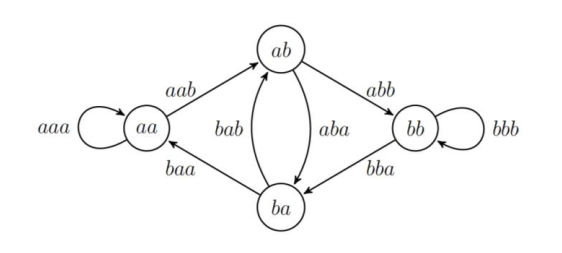
\includegraphics[scale=0.4]{22.png}
\end{figure}

Пример: При помощи графа де Брюина найти слово наименьшей длины,
которое содержит все подслова из множества \\ 
$R=\set{ACT,CTG,TGA,GAC,ACG,CGA}$.

По алгоритму:
\begin{enumerate}[left=0.0em, labelsep=1em, topsep=0.0em, itemsep=0pt, parsep=0.5em]
    \item $V = \set{AC, CT, TG, GA, CG}$ -- вершины графа.
    \item Строим граф.
    \begin{figure}[h]
        \centering
        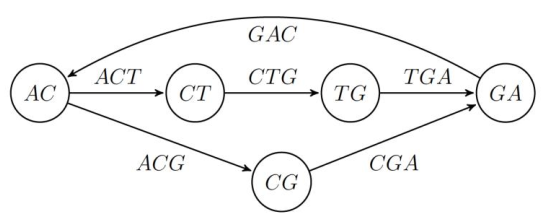
\includegraphics[scale=0.4]{22_2.png}
    \end{figure}
    \item Строим эйлерову цепь: $AC \to CT \to TG \to GA \to AC \to CG \to GA$
    Замечание. Эйлерову цепь начинаем в вершине, из которой выходит на
    одно ребро больше, чем заходит в вершину.
    \item Построенной эйлеровой цепи соответствует слово минимальной длины,
    которое содержит все подслова из $R: ACTGACGA$
    (Cтроим по правилу: $AC+T+G+A+C+G+A$)
\end{enumerate}

